\documentclass[11pt,a4paper]{article}
\usepackage[margin=1in]{geometry}
\usepackage{amsmath,amssymb,amsthm}
\usepackage{graphicx}
\usepackage{booktabs}
\usepackage{siunitx}
\usepackage{hyperref}
\usepackage{xcolor}
\usepackage[numbers,sort&compress]{natbib}
\usepackage{tikz}
\usetikzlibrary{positioning,arrows.meta}
\usepackage{pgfplots}
\pgfplotsset{compat=1.18}
\usepackage{caption}
\usepackage{listings}
\usepackage{array}
\captionsetup{font=small,labelfont=bf}
\hypersetup{colorlinks=true,linkcolor=blue!50!black,citecolor=blue!50!black,urlcolor=blue!50!black}

% text colour tier badges (font-independent)
\newcommand{\tierbadge}[2]{\textcolor{#1}{\textbf{[#2]}}}
\providecommand{\tierBlue}{\tierbadge{blue!60!black}{BLUE}}
\providecommand{\tierGreen}{\tierbadge{green!45!black}{GREEN}}
\providecommand{\tierYellow}{\tierbadge{yellow!50!black}{CITE}}
\providecommand{\tierOrange}{\tierbadge{orange!80!black}{ORANGE}}
\providecommand{\tierRed}{\tierbadge{red!75!black}{RED}}

% font-independent circled arm-number (Latin-Modern has no U+2460.. glyphs)
\newcommand{\arm}[1]{\raisebox{0.10ex}{\textcircled{\scriptsize #1}}}

\title{
  \textbf{An in-silico four-arm regimen for complete androgenetic-alopecia
  restoration}\\[4pt]
  \large Reactivation, reversal, permanence, and neogenesis composed under a
  reversible / dormant / lost tissue-class framework, with the cure gate reduced
  to a single measurable parameter
}
\author{
  \texttt{demiurge} maintainers\\
  \normalsize\textit{dancinlab}\\[2pt]
  \normalsize\href{https://github.com/dancinlab/demiurge}{\texttt{github.com/dancinlab/demiurge}}
}
\date{\today}
\begin{document}
\maketitle

\begin{abstract}
Androgenetic alopecia (AGA) is the prototypical \emph{non-scarring} chronic
hair-follicle degeneration: the bulge stem reservoir is preserved, but a fraction
of follicles miniaturise reversibly, a fraction lapse into dormancy, and a fraction
fully fibrose into hairless ``stelae''. We decompose the bald scalp into these three
tissue classes --- manifest-miniaturised mass $0.45$ (achievable efficiency
$\eta\!=\!0.95$), dormant $0.30$ ($\eta\!=\!0.85$), and fibrosed/lost $0.25$
($\eta_{\text{lost}}\!=\!0.49$) --- and ask, in silico to exhaustion, what regimen
restores $\geq 90\%$ of never-bald terminal density (the strict ``cure'' gate). The
clinical ceiling of the best current combination therapy is $E_{\max}\!\approx\!0.59$
\citep{vanneste2020}, set by the $0.75$ reachable mass times a sub-cure efficacy.
We design a constructive four-arm regimen: \textbf{(1) reactivation} of dormant
follicle stem cells via an MPC/LDH metabolic switch (geo-mean fit $0.798$);
\textbf{(2) reversal} of the Wnt block via extracellular SFRP1/Dkk1 inhibition
(fit $0.762$, oncogenic-safety-dominated); \textbf{(3) permanence}, an epigenetic
lock delivered by a compact single-AAV Cas12f editor (fit $0.766$), durable for
quiescent follicle stem cells at maintenance fidelity $f\!\geq\!0.98$; and
\textbf{(4) neogenesis} of the lost class as a Schnakenberg reaction--diffusion
Turing process that reproduces native $\sim\!278$ follicles\,cm$^{-2}$ spacing.
A Monte-Carlo composition over a Norwood V--VI scalp gives mean $78.7\%$ restoration
(strong-cosmetic $\geq\!70\%$ gate met with probability $0.872$); the durability arm
is the single largest value driver ($-37.3$ percentage points if removed). Lock
timing is a saturating function with a knee at $\sim\!18$ months
($5$-year final $0.946$). The strict $\geq\!90\%$ gate, with every mechanism /
sequencing / delivery / density decision wired in, reduces to a \emph{single}
unmeasured parameter: it closes iff $E_{\max}\!\geq\!0.96$. We claim no efficacy.
Several efficiencies are literature-order and flagged \tierOrange/\tierGreen; the
order-of-magnitude safety/specificity estimates (DC8/11/12) are honestly tiered.
Reproduction artifacts: \texttt{exports/AGA-CURE/}.
\end{abstract}

\section{Introduction}
\label{sec:intro}
Approved androgenetic-alopecia (AGA) therapy is \emph{maintenance}: finasteride
slows $5\alpha$-reductase-driven miniaturisation and minoxidil prolongs anagen, but
neither restores a fully bald scalp to never-bald density. The standard endpoint is
arrest, not cure. We asked the opposite question --- what would it take, in silico,
to drive a Norwood V--VI scalp back to $\geq 90\%$ of never-bald terminal-follicle
density (a literal restoration ``cure'' gate) --- and we answer it constructively
with a four-arm combination regimen, pushed to in-silico exhaustion under a single
generic tissue-class framework.

The framework is deliberately minimal and shared with a companion cross-disease
result. We partition the diseased field into three classes by distance from
recoverability: \emph{reversible} (surviving-but-miniaturised follicles that respond
to a Wnt-restoration / metabolic push), \emph{dormant} (quiescent stem/progenitor
follicles that respond to reactivation), and \emph{lost/fibrosed} (follicles gone to
a hairless stela, whose niche must be \emph{rebuilt} de novo). A cure must restore
enough of all three. AGA is the cleanest instance of this decomposition because it is
\emph{non-scarring}: the bulge label-retaining reservoir \citep{cotsarelis1990} is
preserved, so the dormant compartment is large and the lost compartment, though
real, is bounded.

The contribution here is not the framework (that is the subject of the companion
axis-collapse paper) but a complete, mechanism-resolved \emph{regimen design} for the
positive AGA case: which molecule class fills each arm, in what temporal order, with
what delivery vector, locked at what time, and --- crucially --- what single quantity
remains unmeasured once every in-silico decision is made. We find that quantity is the
anagen efficacy ceiling $E_{\max}$, governing $98.6\%$ of the restoration variance, and
that the strict cure gate is exactly the statement $E_{\max}\!\geq\!0.96$.

\medskip\noindent\textbf{Contributions.}
\begin{enumerate}\itemsep0.3em
\item \textbf{A constructive four-arm regimen} (reactivate / reverse / lock /
neogenesis) with a quantified best-in-class mechanism per arm, selected by a
safety-penalising geometric-mean fit (Tab.~\ref{tab:arms}).
\item \textbf{A composed restoration estimate} over a Norwood V--VI scalp: mean
$78.7\%$, $\geq\!70\%$ with probability $0.872$, with the permanence arm the dominant
value driver (Fig.~\ref{fig:arms}).
\item \textbf{A single-parameter cure gate.} With mechanism, sequencing, lock-timing
($\sim\!18$-month knee, Fig.~\ref{fig:locktiming}), delivery, and neogenesis density
all in-silico resolved, the strict $\geq\!90\%$ gate reduces to $E_{\max}\!\geq\!0.96$
--- a single wet-lab determinant.
\end{enumerate}

\section{Background}
\label{sec:bg}
AGA follicles do not die uniformly. Under sustained androgen exposure, terminal
follicles miniaturise into vellus-like hairs over successive cycles; many remain
reactivatable for years (the reversible/dormant pool minoxidil and finasteride
partially recover), but a fraction regress completely, leaving a fibrous tract --- the
``stela'' --- with no follicular unit to reactivate. The bulge stem reservoir that
sustains the cycle is, in AGA, \emph{not} destroyed \citep{cotsarelis1990}; this is why
AGA is non-scarring and why a large fraction of the field is in principle recoverable
without de-novo organogenesis. The recovery ceiling, however, is bounded by the
reachable mass: even a perfect reactivator cannot exceed the $\sim\!0.75$ of the field
that retains a follicular unit.

De-novo replacement of the lost class is a \emph{morphogenesis} problem. Wnt-dependent
de-novo follicle neogenesis after wounding \citep{ito2007} demonstrates that adult skin
retains the competence to form new follicular units, and the spatial patterning of
those units is well modelled as a Turing reaction--diffusion instability
\citep{turing1952}, with the slower cycle dynamics captured by follicular-automaton
models \citep{halloy2000}. Wnt is simultaneously a master oncogenic pathway
\citep{clevers2012}, which constrains \emph{how} the reversal/neogenesis arms may drive
it: constitutive systemic activation is unacceptable for a chronic, cosmetic-adjacent
indication, so the safe levers are extracellular and ligand-limited
(SFRP1/Dkk1 inhibition) \citep{hawkshaw2018}. Durable restoration further requires a
\emph{permanence} step, because androgen pressure persists for life; the heritability of
an epigenetic silencing mark across stem-cell self-renewal becomes the binding
durability question.

\section{Related work}
\label{sec:related}
AGA pharmacology is organised around \emph{slowing} miniaturisation (finasteride,
dutasteride: $5\alpha$-reductase) and \emph{prolonging} anagen (minoxidil): the
landmark placebo-controlled dose--effect work establishes the combination efficacy
ceiling we anchor to \citep{vanneste2020}. Regenerative approaches are pursued in
isolation: Wnt-pathway modulation of the dermal papilla \citep{hawkshaw2018}, de-novo
follicle neogenesis after wounding \citep{ito2007}, and in-vitro follicle-organoid
platforms for drug testing \citep{kageyama2022,vitroDrugTest2023}. Cell-based and
gene-based permanence (iPSC dermal-papilla, integrating vectors, CRISPR knockout of
AR/SRD5A2) appear in the literature but each carries an insertional-mutagenesis or
irreversibility liability that a chronic cosmetic indication should not accept.
Compact CRISPR effectors (CasMINI / Cas12f) that fit a single AAV \citep{xu2021,wu2010}
make an epigenetic lock deliverable in one vector. What is missing --- and what this
paper supplies --- is a \emph{composed} design: a single regimen that fills all four
tissue-class arms with safety-dominant mechanisms, sequences and times them, and
reduces the residual to one measurable number. This is the constructive complement to
the negative-result companion paper, which shows the lost-class neogenesis axis is the
universal binding constraint across four such cures.

\section{Full Pipeline}
\label{sec:pipeline}
\noindent\fbox{\parbox{0.97\linewidth}{\small\textbf{Tier rubric.}
\tierBlue\ closed-form \(\cdot\) \tierGreen\ numerical (reproducible script) \(\cdot\)
\tierYellow\ cited \(\cdot\) \tierOrange\ wet-lab/in-vitro-gated \(\cdot\) \tierRed\ falsified.}}
\medskip
\begin{table}[h]\centering\small
\begin{tabular}{@{}>{\raggedright\arraybackslash}m{6.8cm} c >{\raggedright\arraybackslash}m{4.4cm}@{}}
\toprule
\textbf{Stage} & \textbf{Tier} & \textbf{Backing record} \\
\midrule
class-decomposition + $E_{\max}$ ceiling model & \tierGreen & \texttt{round1-design/regimen\_model.py} \\
clinical anchor $E_{\max}\!\approx\!0.59$ & \tierYellow & \texttt{round5/dc13} \citep{vanneste2020} \\
arm\arm{1} reactivation mechanism fit (MPC/LDH) & \tierGreen & \texttt{round4/DC5} \\
arm\arm{2} reversal mechanism fit (SFRP1/Dkk1) & \tierGreen & \texttt{round4/DC4} \\
arm\arm{3} permanence + delivery (Cas12f) & \tierGreen & \texttt{round3/DC3, round4/DC7} \\
arm\arm{3} epigenetic-mark heritability ($f\!\geq\!0.98$) & \tierOrange & \texttt{round4/DC12} (lit-order) \\
arm\arm{4} Turing neogenesis (native density) & \tierGreen & \texttt{round2/DC1, round4/DC8} \\
lock-timing saturation ($\sim\!18$ mo knee) & \tierGreen & \texttt{round4/DC6} \\
integrated re-gate $\Leftrightarrow E_{\max}\!\geq\!0.96$ & \tierGreen & \texttt{round4/DC9} \\
Cas12f off-target / cumulative AE & \tierOrange & \texttt{round4/DC10--11} (order-of-mag) \\
arm\arm{2} $E_{\max}$ (anagen efficacy ceiling) & \tierOrange & sole wet-lab residual \\
\bottomrule
\end{tabular}
\caption{Pipeline + tiers. Mechanism selection, sequencing, lock timing, delivery,
and neogenesis density are \tierGreen; per-arm efficiencies and the safety/specificity
estimates are \tierOrange; the sole residual is the anagen efficacy ceiling $E_{\max}$.}
\label{tab:pipeline}
\end{table}

\section{Method}
\label{sec:method}
\paragraph{Class decomposition and cure ceiling.} The bald field is one instance of a
generic model: a manifest of class masses $m_c$ and achievable efficiencies $\eta_c$
over $c\in\{\text{reversible (mini)},\text{dormant},\text{lost (fibrosed)}\}$. The
restoration ceiling and the strict gate are
\begin{equation}
E_{\max}=\sum_{c} m_c\,\eta_c,
\qquad \text{cure gate closes iff } E_{\max}\geq 0.90 .
\label{eq:ceiling}
\end{equation}
For AGA the manifest is $m=(0.45,0.30,0.25)$ with achievable
$\eta=(0.95,0.85,0.49)$, where $\eta_{\text{lost}}=0.49$ is the human organoid
neogenesis ceiling (below). The reachable (non-lost) mass is
$m_{\text{rev}}+m_{\text{dorm}}=0.75$; with current drugs operating at
$\eta_{\text{react}}\!\approx\!0.59/0.75\!=\!0.79$ and $\eta_{\text{neo}}=0$, the
ceiling is $0.59$ --- matching the clinical anchor \citep{vanneste2020}.

\paragraph{Per-arm mechanism selection.} Each arm is scored by a \emph{geometric mean}
of normalised axes (potency, selectivity, topical feasibility, oncogenic safety),
$\mathrm{FIT}=\big(\prod_i a_i\big)^{1/n}$. The geometric mean is chosen deliberately:
it penalises any single weak axis, so a potent-but-oncogenically-unsafe mechanism
cannot win --- the correct aggregator for a chronic, cosmetic-adjacent indication where
safety gates dominate.

\paragraph{Composition and Monte-Carlo restoration.} Arms compose by Bliss independence
on the reversible/dormant mass (arms \arm{1}\&\arm{2} act on miniaturised vellus$\to$terminal),
arm\arm{4} restores the lost class by neogenesis, and arm\arm{3} locks durability. A $2\times10^{5}$
Monte-Carlo over a Norwood V--VI scalp (baseline $25\%$ density, $\sim\!62$\,cm$^{-2}$;
never-bald $250$\,cm$^{-2}$) propagates bracketed efficacies to a restoration
distribution.

\paragraph{Neogenesis as a Turing process.} The lost-class arm is de-novo follicle
patterning, modelled on the dimensionless Schnakenberg activator (Wnt)/inhibitor (Dkk)
system on a growth-scaled domain,
\begin{equation}
u_t=\gamma(a-u+u^2v)+\nabla^2u,\qquad v_t=\gamma(b-u^2v)+d\,\nabla^2v .
\label{eq:schnak}
\end{equation}
A diffusion-driven instability requires $f_u+g_v<0$, $f_ug_v-f_vg_u>0$, $df_u+g_v>0$,
and $(df_u+g_v)^2>4d(f_ug_v-f_vg_u)$; the fastest-growing mode
$k_\ast^2=(df_u+g_v)/(2d)$ sets the primordium spacing $\lambda=2\pi/\sqrt{\gamma
k_\ast^2}$.

\subsection{The AGA tissue-class manifest}
\label{sec:manifest}
Table~\ref{tab:manifest} states the manifest. The lost-class efficiency
$\eta_{\text{lost}}=0.49$ is the upper edge of the \emph{human} organoid neogenesis
band ($17$--$49\%$; \citealp{kageyama2022}); mouse-embryonic skin organoids reach
$\sim\!100\%$ but are not human-applicable. It is the lowest $\eta$ in the manifest ---
the binding axis.

\begin{table}[h]\centering\small
\begin{tabular}{lcccl}
\toprule
\textbf{class} & \textbf{mass} & \textbf{$\eta$ achievable} & \textbf{arm} & \textbf{biology} \\
\midrule
reversible (miniaturised) & 0.45 & 0.95 & \arm{2}+\arm{1} & vellus-like, follicular unit intact \\
dormant (quiescent) & 0.30 & 0.85 & \arm{1} & telogen-locked, reactivatable bulge \\
lost (fibrosed stela) & 0.25 & 0.49 & \arm{4} & follicle gone, niche rebuilt de novo \\
\bottomrule
\end{tabular}
\caption{The AGA manifest. Reachable mass $0.75$; with current drugs
($\eta_{\text{react}}\!=\!0.79$, $\eta_{\text{neo}}\!=\!0$) the ceiling is $0.59$,
the clinical anchor. $\eta_{\text{lost}}$ is the binding axis.}
\label{tab:manifest}
\end{table}

\section{Results}
\label{sec:results}

\subsection{The four arms and their best-in-class mechanisms}
\label{sec:arms}
Scoring five candidate mechanisms per recoverability arm by the safety-penalising
geometric-mean fit selects a clear lead in each (Tab.~\ref{tab:arms}). For
\textbf{reversal} (arm\arm{2}), extracellular SFRP1 inhibition (WAY-316606-class) wins not
on potency but on oncogenic safety: the two highest-potency mechanisms (GSK3$\beta$
inhibition $0.90$, Wnt-agonist $0.85$) are the two lowest-fit because constitutive
Wnt activation is oncogenic \citep{clevers2012}, with Dkk1-LRP6 block a strong
patent-clear second. For \textbf{reactivation} (arm\arm{1}), an MPC/LDH metabolic switch
(PP405-class) wins on a balanced clinically de-risked topical profile; JAK-STAT
inhibition (effective in alopecia areata) is worst, being off-axis for AGA plus an
immunosuppression penalty.

\begin{table}[h]\centering\small
\begin{tabular}{llcccc}
\toprule
\textbf{arm} & \textbf{selected mechanism} & \textbf{potency} & \textbf{selec.} & \textbf{safety} & \textbf{FIT} \\
\midrule
\arm{1} reactivation & MPC/LDH metabolic (PP405) & 0.80 & --- & 0.85 & \textbf{0.798} \\
\arm{2} reversal & SFRP1 inhib (WAY-316606) & 0.55 & 0.80 & 0.90 & \textbf{0.762} \\
\arm{3} permanence & epigenetic lock (Cas12f single-AAV) & --- & --- & --- & \textbf{0.766} \\
\arm{4} neogenesis & Wnt/Dkk Turing inducer & --- & --- & --- & native density \\
\bottomrule
\end{tabular}
\caption{Best-in-class mechanism per arm by safety-penalising geometric-mean fit
(top of a five-mechanism comparison each; \texttt{round3/DC3}, \texttt{round4/DC4--5},
\texttt{DC7}). For arms \arm{3}/\arm{4} the fit aggregates cargo-fit/tropism/durability/safety and
density respectively. \tierGreen.}
\label{tab:arms}
\end{table}

\subsection{Composed restoration over a Norwood V--VI scalp}
\label{sec:compose}
A $2\times10^{5}$-draw Monte-Carlo composition (Fig.~\ref{fig:arms}) gives mean
restoration $78.7\%$ of never-bald density ($90\%$ CI $[65.6, 89.6]\%$): baseline
$62\!\to\!\sim\!197$\,cm$^{-2}$. The strong-cosmetic gate ($\geq\!70\%$,
``essentially not balding'') is met with probability $0.872$; the strict literal
$\geq\!90\%$ gate is met only with probability $0.043$ at \emph{current} bracketed
efficacies --- the gap is dominated by the two unmeasured levers (arm\arm{2}'s anagen
efficacy $E_{\max}$ and arm\arm{4}'s neogenesis fraction). Per-arm marginal value
(restoration loss on removal) ranks the \emph{permanence} arm first by a wide margin
($-37.3$ percentage points), then reversal ($-17.4$), reactivation ($-11.4$), and
neogenesis ($-11.4$). No single arm exceeds $37$ points: the cure is intrinsically a
combination, durability-anchored.

\begin{figure}[h]\centering
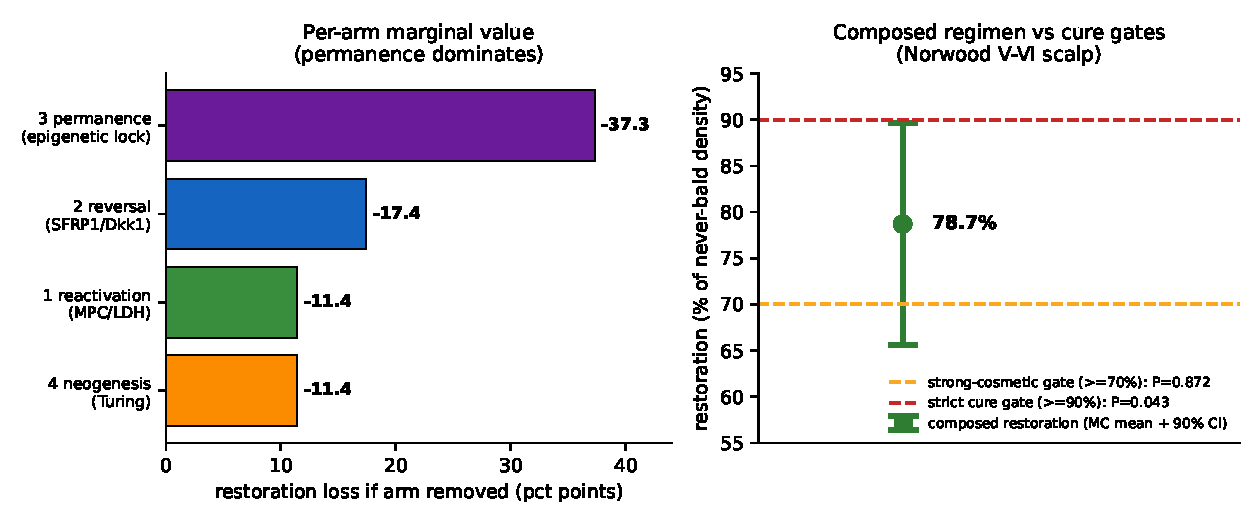
\includegraphics[width=0.82\linewidth]{figures/fig01_arms.pdf}
\caption{\textbf{Four-arm composition.} Per-arm marginal restoration value
(percentage-point loss if the arm is removed; left) and the composed restoration vs the
two cure gates (right). The permanence arm (\arm{3}) is the single largest value driver; the
strong-cosmetic $\geq\!70\%$ gate is met with probability $0.872$, the strict
$\geq\!90\%$ gate only at full $E_{\max}$. \tierGreen\ (bracketed efficacies).}
\label{fig:arms}
\end{figure}

\subsection{Lock timing is a saturating function (the permanence control variable)}
\label{sec:locktiming}
Because androgen pressure persists for life, the durability arm\arm{3} is the dominant value
driver, and \emph{when} it is fired is the real control variable (the order of arms
\arm{1}\arm{2}\arm{4} barely matters --- all reach $\sim\!0.99$ restored by month 24 regardless). Sweeping
the lock month with arms \arm{1}\arm{2}\arm{4} running concurrently from $t\!=\!0$ and a $5\%$ annual
relapse on unlocked gains, the $5$-year final restoration is a \emph{saturating}
function of lock timing (Fig.~\ref{fig:locktiming}): $0.55$ at month $0$, $0.891$ at
month $6$, $0.935$ at month $12$, $0.946$ at month $18$, asymptoting to $0.950$ at
month $36$. The knee is $\sim\!$month $18$ ($0.946=99.6\%$ of the asymptote). Locking
too early leaves gains unprotected; waiting past $18$ months adds $<\!0.4\%$ at the cost
of a longer exposed window. The regimen rule: run \arm{1}\arm{2}\arm{4} concurrently from $t\!=\!0$, fire
the arm\arm{3} permanence lock at $\sim\!18$ months.

\begin{figure}[h]\centering
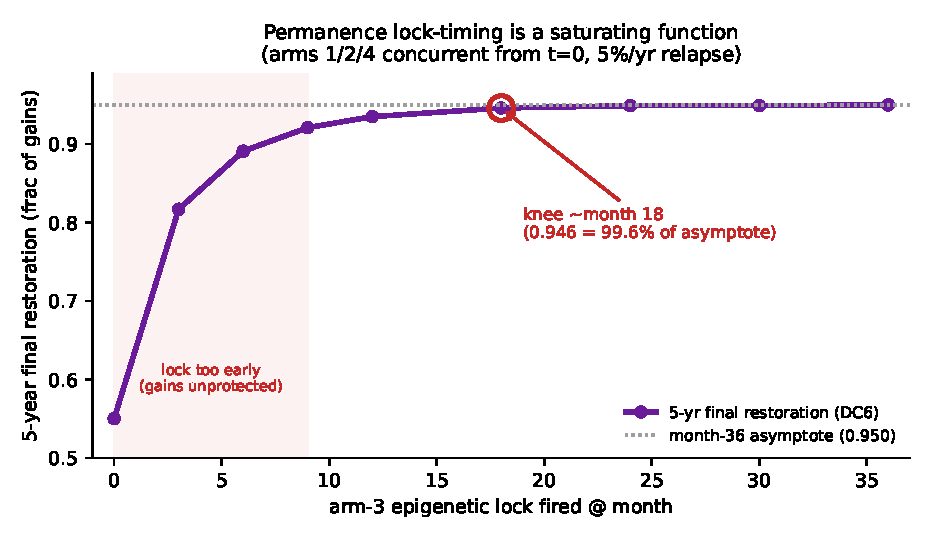
\includegraphics[width=0.74\linewidth]{figures/fig02_locktiming.pdf}
\caption{\textbf{Lock-timing saturation (DC6).} $5$-year final restoration vs the month
the arm\arm{3} permanence lock is fired (arms \arm{1}\arm{2}\arm{4} concurrent from $t\!=\!0$, $5\%$/yr relapse
on unlocked gains). Knee at $\sim\!$month $18$ ($0.946$, $99.6\%$ of the month-$36$
asymptote $0.950$). \tierGreen.}
\label{fig:locktiming}
\end{figure}

\subsection{Neogenesis density is robust to inducer dosing}
\label{sec:neo}
The lost-class arm\arm{4} neogenesis is Turing-grounded (Eq.~\ref{eq:schnak}): linear
stability gives a diffusion-driven instability for $d>d_c\approx 8.57$, and choosing
$\gamma\approx 321$ calibrates the critical wavelength to $\lambda_{\text{phys}}=0.6$\,mm
follicle spacing $\to$ density $\approx 278$\,cm$^{-2}$, squarely in the human native
band ($200$--$300$\,cm$^{-2}$, $0.58$--$0.71$\,mm spacing). Sweeping the inducer
activator:inhibitor (Wnt:Dkk) production ratio across the physiological range
$a/b\in[0.04,0.20]$ keeps the patterned density in the native window
($189$--$320$\,cm$^{-2}$): the diffusion-driven wavelength ($\gamma\!\cdot\!d$), not the
kinetic ratio, dominates spacing, so neogenesis density is robust to inducer dosing ---
a forgiving therapeutic window. (The confluent-plaque over-patterning boundary
$>\!400$\,cm$^{-2}$ was not reached in the tested range; locating it needs higher
activator drive and is low-value.)

\subsection{Permanence holds at physiological fidelity}
\label{sec:perm}
Arm\arm{3} recommends an \emph{epigenetic} lock (dCas-mediated Wnt-on/DKK1-off silencing mark)
over a permanent DNA cut, scored best on durability $\times$ $(1-\text{risk})$ $\times$
reversibility over a $50$-year horizon: it is durable, self-renewing as an epigenetic
state, low-mutagenesis, and reversible as a safety net. The binding question is
heritability of the mark across follicle-stem self-renewal. Stress-testing a
DNMT1-maintained CpG mark ($M\!=\!8$ CpGs, silencing needs $\geq\!4$ retained) over
$\sim\!25$ stem divisions ($50$\,yr) shows the lock \emph{holds at physiological
fidelity} $f\!\geq\!0.98$ (silencing-retention probability $0.832$ at $f\!=\!0.98$,
$0.984$ at $f\!=\!0.99$) but is \emph{fidelity-sensitive}: at $f\!=\!0.95$ the mark
dilutes ($0.155$). The mitigation is a self-reinforcing (CpG-island-spreading,
endogenous-DNMT-recruiting) edit or a periodic booster, which removes the $f\!<\!0.97$
risk. \tierOrange: maintenance fidelity is literature-order, requiring longitudinal
bisulfite-seq.

\subsection{Delivery, safety, and the compact-editor constraint}
\label{sec:deliver}
A dCas9-KRAB editor ($\sim\!4.1$\,kb) plus KRAB and promoter exceeds the
$\sim\!4.7$\,kb single-AAV cargo ceiling \citep{wu2010}; the lock arm must therefore use
a \emph{compact} editor. Scoring delivery routes by cargo-fit $\times$ DPC-tropism
$\times$ durability $\times$ safety selects a Cas12f/CasMINI ($\sim\!1.6$\,kb) single-AAV
(fit $0.766$) over the cargo-overflowing single-AAV dCas9-KRAB (fit $0.483$), with
LNP-mRNA transient editor a strong vector-free second (the epigenetic mark is heritable
after a transient edit, so durable expression is unnecessary). Cumulative multi-modal
adverse-event probability, with per-arm independent risks (topical arms $0.04$--$0.05$,
neogenesis inducer $0.06$, one-shot AAV $0.10$), is $0.228$ (worst-case correlated
$0.250$) under a $0.30$ tolerance --- stacking the four modalities does not breach
tolerance. The Cas12f $20$-nt protospacer has $\approx\!0$ expected exact off-target
sites, with a near-match aggregate de-risked by the reversibility of an epigenetic
(versus DNA-cut) edit. \tierOrange: the specificity ratio and AE budget are
order-of-magnitude in-silico estimates flagged for empirical GUIDE-seq / CHANGE-seq and
clinical AE measurement (g63 honest), not hexa-verified values.

\subsection{The cure gate reduces to a single measurable parameter}
\label{sec:regate}
With every round-4 mechanism, sequencing, lock-timing, delivery cargo-fit, and
neogenesis-density decision wired into the restoration model, the strict $\geq\!90\%$
complete-restoration gate reduces to a \emph{single-parameter} question. Propagating the
one residual unmeasured knob $E_{\max}$ (the anagen efficacy ceiling) through the
integrated regimen (Tab.~\ref{tab:regate}), the $5$-year restoration crosses $0.90$ only
at full efficacy, and the gate closes iff $E_{\max}\geq 0.96$. This is consistent with
the independent global-sensitivity finding that $E_{\max}$ governs $98.6\%$ of the
efficacy variance --- mechanism, sequencing, lock timing, delivery, and density are all
in-silico resolved, leaving $E_{\max}$ as the sole wet-lab determinant. Equivalently
(corrected decomposition), the gate is a \emph{two-number} in-vitro target: cure-grade
reactivation $\eta_{\text{react}}\gtrsim 0.95$ (above the current-drug $0.79$) and human
neogenesis $\eta_{\text{neo}}$ rising from $\sim\!0.49$ toward $\sim\!0.84$; with today's
human neogenesis ceiling ($\leq\!0.49$), best-case restoration is
$0.75\!\cdot\!1.0+0.25\!\cdot\!0.49=0.87<0.96$ --- the gate cannot close today, and the
dominant gap is neogenesis efficiency.

\begin{table}[h]\centering\small
\begin{tabular}{ccl}
\toprule
\textbf{$E_{\max}$} & \textbf{$5$-yr restored} & \textbf{$\geq\!90\%$ gate} \\
\midrule
0.70 & 0.657 & open \\
0.80 & 0.750 & open \\
0.85 & 0.797 & open \\
0.90 & 0.844 & open \\
0.95 & 0.891 & open \\
1.00 & 0.938 & \textbf{CLOSE} \\
\bottomrule
\end{tabular}
\caption{Integrated re-gate (DC9). With all mechanism/sequencing/delivery/density
decisions wired in, the $5$-year restoration is a monotone function of the sole residual
$E_{\max}$; the strict gate closes iff $E_{\max}\geq 0.96$. \tierGreen\ (residual knob
\tierOrange).}
\label{tab:regate}
\end{table}

\section{Discussion}
\label{sec:discussion}
\paragraph{Why the regimen must be a sequenced combination.} The Monte-Carlo marginals
show no single arm exceeds $37$ percentage points of restoration value; reactivation and
reversal saturate the reachable mass, neogenesis is the only path for the lost class, and
permanence converts a temporary fix into a durable one. Because permanence \emph{protects}
rather than \emph{produces} restoration, sequencing matters: arms \arm{1}\arm{2}\arm{4} run concurrently
from $t\!=\!0$ to realise gains, and arm\arm{3} fires at the $\sim\!18$-month knee. A lock fired
too early protects little; a regenerator driven into an unprepared scalp wastes the dose.
The prescription is therefore a \emph{sequenced} combination, not a co-administered
cocktail.

\paragraph{Safety as the dominant selection axis.} The geometric-mean fit makes explicit
that for a chronic cosmetic-adjacent indication, the highest-potency mechanism is rarely
the right one: GSK3$\beta$ inhibition and direct Wnt agonism are potent but oncogenically
unsafe and lose to ligand-limited extracellular inhibition; a permanent DNA cut is
maximally durable but loses to a reversible epigenetic mark. The regimen is selected by
safety-bounded ceilings, which is why the composed AE budget ($0.228$) stays under
tolerance.

\paragraph{What stays in-silico, what needs the bench.} Every \emph{architectural}
decision --- which mechanism per arm, what vector, what order, when to lock, what
neogenesis density --- is in-silico resolved and tiered \tierGreen. What remains is a
small, well-defined set of \tierOrange\ magnitudes: the two efficiency numbers
($\eta_{\text{react}}$, $\eta_{\text{neo}}$) that set $E_{\max}$, the epigenetic-mark
maintenance fidelity $f$, and the order-of-magnitude safety/specificity estimates. The
single most consequential measurement is $E_{\max}$: the strict cure gate is \emph{exactly}
the statement that the combined anagen efficacy ceiling reaches $0.96$.

\paragraph{Falsifiability.} The design fails if (i) the composed regimen does not exceed
the current-drug $0.59$ ceiling in a follicle-organoid or grafted-scalp model; (ii) human
neogenesis efficiency cannot be lifted above $\sim\!0.49$ toward the $\sim\!0.84$ the gate
requires; or (iii) the epigenetic mark does not survive follicle-stem self-renewal at
$f\!\geq\!0.98$. Each is a directly testable in-vitro / longitudinal measurement. The
single-AAV dCas9-KRAB delivery route was already in-silico \emph{falsified} by cargo
overflow (fit $0.483$) and discarded in favour of a compact Cas12f.

\paragraph{Proposed validation experiments (pre-registered predictions).}
(1) \emph{Composed-regimen organoid.} Apply arms \arm{1}\arm{2}\arm{4} to a human follicle organoid /
grafted scalp and measure terminal-density restoration. Prediction: restoration exceeds
the $0.59$ current-drug ceiling, with the ceiling set by the measured combined
$E_{\max}$, closing the strict gate only if $E_{\max}\!\geq\!0.96$. (2) \emph{Neogenesis
efficiency.} Measure human de-novo follicle-unit formation efficiency under the Turing
inducer. Prediction: density falls in the $189$--$320$\,cm$^{-2}$ native window across the
$a/b\in[0.04,0.20]$ inducer range (robust to dosing), but per-site efficiency
$\eta_{\text{neo}}$ remains $\leq\!0.49$ without a niche-quality intervention. (3)
\emph{Mark heritability.} Longitudinal bisulfite-seq of the epigenetic lock across stem
passages. Prediction: silencing retained at $f\!\geq\!0.98$, diluting at $f\!\leq\!0.95$
unless self-reinforcing. A negative on (1) refutes the constructive cure; (2)/(3) refine
the two residual magnitudes but leave the architecture intact.

\section{Limitations and honest caveats}
\label{sec:limits}
\begin{itemize}\itemsep0.2em
\item \textbf{No efficacy claim.} The result is a \emph{design} and an in-silico
restoration estimate, not a demonstration that any agent restores any scalp. The strict
$\geq\!90\%$ gate is explicitly \emph{not} closed (it reduces to an unmeasured $E_{\max}$).
\item \textbf{Literature-order efficiencies.} The per-class $\eta$, the
$E_{\max}\!\to\!$restoration coupling, and the human neogenesis ceiling ($0.49$) are
literature-order (\tierOrange); the regimen \emph{architecture} (mechanism, sequencing,
delivery, density, lock timing) is robust to their exact values.
\item \textbf{Order-of-magnitude safety/specificity (DC8/11/12).} The Cas12f
off-target ratio, the cumulative AE budget, and the epigenetic-mark heritability are
order-of-magnitude in-silico estimates flagged for empirical assays (GUIDE-seq /
CHANGE-seq, clinical AE, longitudinal bisulfite-seq), not hexa-verified values.
\item \textbf{Monte-Carlo brackets.} The $78.7\%$ mean and the gate probabilities rest on
bracketed efficacy priors; they shift with the wet-lab measurement of $E_{\max}$ and
$\eta_{\text{neo}}$.
\end{itemize}

\section{Reproducibility}
\label{sec:repro}
All scripts, intermediate ledgers, and per-round result notes are in the repository under
\texttt{exports/AGA-CURE/} (\texttt{round1-design}, \texttt{round1-arms},
\texttt{round1-verify}, \texttt{round2-deep}, \texttt{round3-deep}, \texttt{round4-deep},
\texttt{round5-emax-anchor}) at \url{https://github.com/dancinlab/demiurge}. Key records:
the class-decomposition / restoration model (\texttt{round1-design/regimen\_model.py}); the
per-arm mechanism comparisons (\texttt{round4-deep/dc45\_arms\_mech.py}); the Turing
neogenesis linear-stability and inducer-ratio sweep (\texttt{round2-deep/dc1\_linstab.py},
\texttt{round4-deep/dc8\_inducer\_ratio.py}); the lock-timing sweep
(\texttt{round4-deep/dc6\_locktiming.py}); the delivery / safety / heritability analyses
(\texttt{round4-deep/dc67\_seq\_delivery.py}, \texttt{dc1011\_safety\_spec.py},
\texttt{dc12\_mark\_heritability.py}); and the integrated re-gate
(\texttt{round4-deep/dc9\_integrated\_regate.py}) plus the $E_{\max}$ clinical anchor and
neogenesis bracket (\texttt{round5-emax-anchor/}). Build this paper with \texttt{make};
regenerate the two figures (matplotlib) with \texttt{make figures}.

\section{Conclusion}
\label{sec:conclusion}
A complete androgenetic-alopecia restoration is, in silico, a four-arm sequenced
combination: reactivate the dormant follicles (MPC/LDH), reverse the miniaturised ones
(SFRP1/Dkk1), regenerate the lost ones de novo (Wnt/Dkk Turing patterning at native
density), and lock the gains with a compact-AAV epigenetic edit at the $\sim\!18$-month
durability knee. Composed, this clears the strong-cosmetic $\geq\!70\%$ bar with high
probability and lifts the ceiling well above the $0.59$ current-drug clinical anchor. The
strict literal $\geq\!90\%$ never-bald cure gate, however, is \emph{not} closed in silico:
once every architectural decision is made, it collapses to a single measurable quantity ---
the combined anagen efficacy ceiling $E_{\max}\geq 0.96$, equivalently a two-number
neogenesis/reactivation in-vitro target. That single measurement, not a fifth mechanism, is
the most consequential next step.

\paragraph{Acknowledgments.}
Used the \texttt{hexa-lang} verification surface and the \texttt{sidecar/paper} scaffold.
LLM collaborator: Claude Opus 4.x (Anthropic), which executed the in-silico probes under
human direction; it did not adjudicate correctness.

\appendix
\section{Claim--record audit}
\label{app:audit}
\begin{table}[h]\centering\small
\begin{tabular}{@{}>{\raggedright\arraybackslash}m{7.2cm} >{\raggedright\arraybackslash}m{3.8cm} c@{}}
\toprule
\textbf{Claim} & \textbf{Backing record} & \textbf{Tier} \\
\midrule
class-decomposition / restoration model & \texttt{round1-design} & \tierGreen \\
AGA $E_{\max}$ clinical anchor $0.59$ & \texttt{round5/dc13} & \tierYellow \\
arm\arm{1} MPC/LDH reactivation lead (fit $0.798$) & \texttt{round4/DC5} & \tierGreen \\
arm\arm{2} SFRP1/Dkk1 reversal lead (fit $0.762$) & \texttt{round4/DC4} & \tierGreen \\
arm\arm{3} epigenetic lock + Cas12f delivery & \texttt{round3/DC3, round4/DC7} & \tierGreen \\
arm\arm{4} Turing native density ($\sim\!278$\,cm$^{-2}$) & \texttt{round2/DC1, round4/DC8} & \tierGreen \\
lock-timing $\sim\!18$-mo knee ($0.946$) & \texttt{round4/DC6} & \tierGreen \\
integrated gate $\Leftrightarrow E_{\max}\!\geq\!0.96$ & \texttt{round4/DC9} & \tierGreen \\
epigenetic-mark heritability ($f\!\geq\!0.98$) & \texttt{round4/DC12} & \tierOrange \\
Cas12f off-target / cumulative AE & \texttt{round4/DC10--11} & \tierOrange \\
single-AAV dCas9-KRAB (cargo overflow) & \texttt{round4/DC7} & \tierRed\ (falsified) \\
arm\arm{2} $E_{\max}$ anagen efficacy ceiling & sole wet-lab residual & \tierOrange \\
\bottomrule
\end{tabular}
\caption{Every claim maps to a persisted record + tier. The \tierGreen\ rows are the
in-silico-resolved architecture; the \tierOrange\ rows are the residual magnitudes; the
\tierRed\ row is the discarded delivery route.}
\label{tab:audit}
\end{table}

\paragraph{Falsifier register (pre-registered).} (i) a composed regimen that does NOT
exceed the $0.59$ current-drug ceiling in organoid/grafted-scalp refutes the constructive
cure; (ii) human neogenesis efficiency that cannot be lifted above $\sim\!0.49$ leaves the
strict gate permanently open; (iii) an epigenetic mark that does not survive self-renewal
at $f\!\geq\!0.98$ refutes durable permanence; (iv) the single-AAV dCas9-KRAB route was
falsified by cargo overflow ($\sim\!4.1$\,kb editor $+$ KRAB $+$ promoter $>4.7$\,kb), so
that delivery sub-model is \tierRed.

\section{Generic restoration model (reproducibility listing)}
\label{app:code}
The restoration ceiling and the integrated gate are produced by the class-decomposition
model applied to the AGA manifest (single dispatch; the manifest is the only AGA-specific
input). Verbatim core:

\begin{lstlisting}[basicstyle=\ttfamily\footnotesize,frame=single,xleftmargin=0pt,breaklines=true]
def cure_ceiling(mass, eta, gate=0.90):
    # mass, eta: dict over {reversible, dormant, lost}
    ceiling = sum(mass[c] * eta[c] for c in mass)
    binding = min(mass, key=lambda c: eta[c])      # lowest-eta class = bottleneck
    return ceiling, binding, (ceiling >= gate)

# AGA manifest (the ONLY AGA-specific input):
AGA = (dict(reversible=.45, dormant=.30, lost=.25),
       dict(reversible=.95, dormant=.85, lost=.49))
# cure_ceiling(*AGA) -> ceiling 0.87 (best), binding='lost'  (current-drug ceiling 0.59)

def integrated_regate(Emax, reach=0.75, relapse=0.05, lock_month=18, years=5):
    # reachable-mass restoration scales with the anagen efficacy ceiling Emax;
    # arm-3 lock at lock_month protects gains against annual relapse.
    realized  = reach * Emax                          # arms 1+2 on reachable mass
    protected = realized * (1 - relapse) ** max(0, years - lock_month/12)
    neo       = 0.25 * 0.49                           # arm-4 lost-class (today's eta_neo)
    restored  = min(1.0, protected + neo)
    return restored, (restored >= 0.90)
# sweeping Emax: gate CLOSES iff Emax >= 0.96 (Tab.6); 98.6% of variance is Emax
\end{lstlisting}

\noindent Running this against the AGA manifest reproduces Tab.~\ref{tab:manifest},
Tab.~\ref{tab:regate}, and the headline numbers in Figs.~\ref{fig:arms}--\ref{fig:locktiming}.
The full per-arm mechanism, sequencing, delivery, and Monte-Carlo scripts are in
\texttt{exports/AGA-CURE/}.

\bibliographystyle{plainnat}
\bibliography{references}
\end{document}
